\documentclass[12pt]{book}

\usepackage[toc]{glossaries}
\usepackage[margin=1in]{geometry}
\usepackage{hyperref}
\usepackage{listings}
\usepackage{tikz}
\usepackage{url}

\hypersetup{
  colorlinks=true,
  allcolors=blue,
}

\title{Pioneers in Engineering \\ Kit Software Documentation}
\author{PiE Software Engineering Team \\ \url{software@pioneers.berkeley.edu}}
\date{\today}

% Glossary
\makeglossaries
\newglossaryentry{gamepad}{name=gamepad, description={is a general term for controller (typically \href{https://www.xbox.com/en-US/xbox-one/accessories/controllers/xbox-black-wireless-controller}{Xbox})}}
\newglossaryentry{smartsensor}{name={Smart Sensor}, description={is the protocol used for device-to-SBC communication}}
\newglossaryentry{smartdevice}{name={Smart Device}, description={is a device that implements the Smart Sensor protocol}}
\newacronym{sbc}{SBC}{Single Board Computer}
\newglossaryentry{raspi}{name={Raspberry Pi}, description={is the current SBC used to control each robot}}
\newglossaryentry{arduino}{name={Arduino}, description={is a family of single-board microprocessors for building digital devices (PiE currently uses the Arduino Pro Micro for Smart Sensors)}}
\newglossaryentry{image}{name={image}, description={is a snapshot of the persistent state of a computer system (this is typically a copy of the disk, and makes robot replication easy)}}
\newglossaryentry{thread}{name={thread}, description={is the execution of a stream of instructions}}
\newglossaryentry{multithreading}{name={multithreading}, description={is the use of multiple threads running concurrently to appear to accomplish several tasks simultaenously}}
\newglossaryentry{blocking}{name={blocking}, description={describes a programming interface that suspends execution until some condition is met (for example, a queue with a blocking dequeue operation will ``block'' the thread of execution if the queue is empty at the time it is read; the queue will unblock once another thread or coroutine enqueues an item)}}
\newglossaryentry{asyncio}{name={async I/O}, description={is a style of programming where, instead of explicitly managing multiple threads, programs are written to respond to events}}
\newglossaryentry{bbb}{name={Beaglebone Black}, description={was an SBC developed by Texas Instruments used before the Raspberry Pi}}
\newglossaryentry{process}{name={process}, description={consists of one or more threads and a memory space (in general, sharing data between processes is difficult)}}
\newacronym{gil}{GIL}{Global Interpreter Lock}
\newglossaryentry{gls-gil} {
  name={Global Interpreter Lock},
  description={
    is a lock in many Python implementations that must be held whenever interacting with Python objects (for reference-counting and garbage collection reasons).
    In vanilla CPython, this means that multithreading cannot take advantage of using multiple cores simultaenously, bottlenecking performance.
    However, there are ways to circumvent the GIL (see multiprocessing, Cython)
  },
}
\newacronym{os}{OS}{Operating System}
\newglossaryentry{gls-os}{
  name={operating system},
  description={
    is a low-level software layer responsible for managing computing resources like memory, disk, CPU time, and providing convenient abstractions like processes
  }
}

% Code styling
\definecolor{silver}{gray}{0.96}
\definecolor{dark-gray}{gray}{0.5}
\definecolor{cyan}{rgb}{0.3, 0.6, 0.6}
\definecolor{light-blue}{rgb}{0.2, 0.4, 0.6}
\definecolor{yellow}{rgb}{0.6, 0.5, 0.3}
\definecolor{red}{rgb}{0.8, 0.4, 0.4}
\lstdefinestyle{light}{
  breaklines=true,
  showstringspaces=false,
  captionpos=b,
  showtabs=false,
  tabsize=4,
  backgroundcolor=\color{silver},
  basicstyle=\ttfamily,
  keywordstyle=\bfseries\color{light-blue},
  commentstyle=\color{dark-gray},
  identifierstyle=\color{cyan},
  stringstyle=\color{yellow},
  numberstyle=\ttfamily,
}
\lstset{framextopmargin=0.2em, framexbottommargin=0.2em,
        xleftmargin=0.3em, framexleftmargin=0.3em,
        frame=single, framerule=0pt, escapechar=@, style=light}

\begin{document}
  \frontmatter
  \maketitle
  \tableofcontents

  \mainmatter

  \chapter{Introduction}

  \section{Motivation}

  \href{https://pierobotics.org}{Pioneers in Engineering} (PiE) is a nonprofit run by the students of University of California, Berkeley to promote STEM\footnote{Science, technology, engineering, and mathematics.} education.
  PiE's outreach primarily takes the form of a twelve-week-long robotics competition among around twenty Bay Area high schools every spring.

  Given the audience we serve, there are some core tenets

  \begin{enumerate}
    \item
      \textbf{The kit should be easy to build, program, and debug.}
      Many students in our target audience---and even many new PiE staff---are programming novices.

    \item
      \textbf{The kit should be highly performant.}
      When a student moves the joystick on her controller, it should feel as if the robot responds instantly.

    \item
      \textbf{The kit should handle faults gracefully.}
      Errors are a fact of life (and perhaps even more so for robotics, where we need to interact with the physical world).
      Hardware will break and code will contain bugs.
      However, with careful design and automated monitoring, we can know when components break and prevent failures from cascading.

    \item
      \textbf{The kit should be backwards-compatible.}
      If we can avoid it, we should not
  \end{enumerate}

  \section{High-Level Architecture}

  \section{Workflow}

  \subsection{Version Control}

  First,

  \subsection{Testing}

  \subsection{Versioning}

  Every ``snapshot'' of each project is associated with a unique \textbf{version number}.
  In Git, we represent this with a

  For more information, consult the \textsc{Pipeline} subproject under \textsc{DevOps}.

  \chapter{Runtime}

  \textsc{Runtime} is a Python application that runs on each robot to manage sensors and actuators, communicate with the field, and execute student code.

  \section{Architecture}

  \begin{figure}[!htbp]
    \centering
    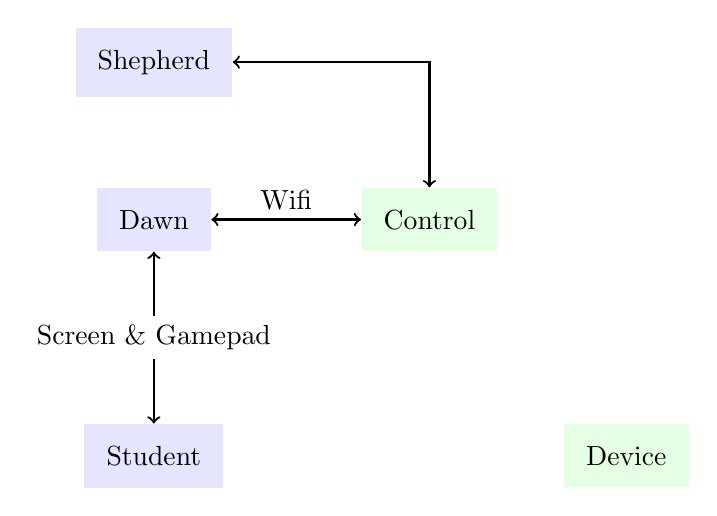
\begin{tikzpicture}
      \node[inner sep=8pt, fill=blue!10] (shepherd) at (0, 2) {Shepherd};
      \node[inner sep=8pt, fill=blue!10] (dawn) at (0, 0) {Dawn};
      \node[inner sep=8pt, fill=blue!10] (student) at (0, -3) {Student};
      \node[inner sep=8pt, fill=green!10] (control) at (3.5, 0) {Control};
      \node[inner sep=8pt, fill=green!10] (devices) at (6, -3) {Device};

      \draw[<->, thick] (student.north) -- (dawn.south) node[midway, fill=white] {Screen \& Gamepad};
      \draw[<->, thick] (dawn.east) -- (control.west) node[midway, above] {Wifi};
      \draw[<->, thick] (shepherd.east) -| (control.north);
    \end{tikzpicture}
    \caption{High-level Runtime architecture.}
    \label{fig:runtime-architecture}
  \end{figure}

  \section{Networking}

  First and foremost, for

  \section{Journal}

  Logs, metrics, and monitors are the tools with which we pinpoint failures and measure performance.
  In a toy program, you might add print statements to trace the flow of execution and watch the data as it is transformed.
  However, for a system as complex and with as many modules as Runtime, we need a more rigorous approach for collecting diagnostic information---this is the purpose of the Runtime \texttt{journal} module.

  The journal is essentially a structured logging layer built on top of Python's built-in \texttt{logging} module.\footnote{Like \href{https://github.com/trentm/node-bunyan}{\texttt{node-bunyan}}.}
  However, unlike conventional logs, which are human-readable strings of text, \href{https://stackify.com/what-is-structured-logging-and-why-developers-need-it/}{structured logs} are written in machine-readable formats like \href{https://www.json.org/}{JSON}.
  This is useful because

  \begin{lstlisting}[gobble=4]
    python -m runtime | python -m runtime.journal
  \end{lstlisting}

  \section{Devices}

  \section{Testing}

  \chapter{DevOps}

  \textsc{DevOps} is a software support project in PiE that performs a number of critical functions for ensuring a working kit:
  \begin{enumerate}
    \item Managing the code build and deployment infrastructure (currently, this is \href{https://travis-ci.org/pioneers/PieCentral}{TravisCI}).
    \item Deploying Runtime and a custom \gls{os} \gls{image} to dozens of \gls{raspi} microSD cards, both for student kits and internal use.
    \item Configuring and monitoring the networking infrastructure.
  \end{enumerate}

  The name is a portmanteau of \textsc{Dev} and \textsc{Ops}, which are short for ``Developer'' and ``Operations,'' respectively.

  One analogy for thinking about DevOps is that the project is the ``glue'' for binding the other projects together.
  Without DevOps, there would be no staff for shipping code from GitHub to kit.

  \section{Fabric}

  Fabric is a software layer that provides support for the PiE software stack.
  Essentially, it's a collection of shell scripts and service configuration files that provides additional customization from the stock release of Raspbian:
  \begin{itemize}
    \item A custom Docker \texttt{runtime} image (based off of \texttt{alpine} Linux) with all the necessary Python dependencies.
    \item A \texttt{fabric} command-line tool for starting, stopping, updating, and checking the status of the \texttt{runtime} Docker container.
    \item Networking configuration files for connecting to the field and team router.
    \item \texttt{systemd} services for starting \texttt{runtime} on boot.
  \end{itemize}

  \section{Pipeline}

  The Pipeline is a subproject for building and deploying software artifacts.

  \section{Networking}

  \chapter{Shepherd}

  \textsc{Shepherd} is the field control software.

  \chapter{Dawn}

  \textsc{Dawn} is a code editor and user interface for interacting with a robot.
  This \href{https://electronjs.org/}{Electron} app\footnote{Electron is essentially a stripped-down version of the Chromium web browser, so developing for Dawn amounts to platform-agnostic web development.} is written in NodeJS, and runs in Windows, macOS, and Linux desktop environments.

  \printglossaries
  \glsaddall
\end{document}
